\section{Details of Experiments on OC20}
\label{appendix:sec:oc20}


\subsection{Detailed Description of OC20 Dataset}
\label{appendix:subsec:oc20_dataset_details}
The dataset consists of larger atomic systems, each composed of a molecule called adsorbate placed on a slab called catalyst.
Each input contains more atoms and more diverse atom types than QM9 and MD17.
The average number of atoms in a system is more than 70, and there are over 50 atom species.
The goal is to understand interaction between adsorbates and catalysts through relaxation.
%Specifically, an adsorbate is first placed on top of a catalyst at heuristically determined locations in order to form initial structure (IS).
An adsorbate is first placed on top of a catalyst to form initial structure (IS).
The positions of atoms are updated with forces calculated by density function theory until the system is stable and becomes relaxed structure (RS).
The energy of RS, or relaxed energy (RE), is correlated with catalyst activity and therefore a metric for understanding their interaction.
We focus on the task of initial structure to relaxed energy (IS2RE), which predicts relaxed energy (RE) given an initial structure (IS).
%We focus on the task of initial structure to relaxed energy (IS2RE), which is to predict the energy of a relaxed structure (RS) given its initial structure (IS).
There are 460k, 100k and 100k structures in training, validation, and testing sets, respectively.
%%%Performance is measured in MAE and energy within threshold (EwT), the percentage in which predicted energy is within 0.02~eV of ground truth energy.
%%%In validation and testing sets, there are four sub-splits containing in-distribution adsorbates and catalysts (ID), out-of-distribution adsorbates (OOD-Ads), out-of-distribution catalysts (OOD-Cat), and out-of-distribution adsorbates and catalysts (OOD-Both).



\subsection{Training Details}
\label{appendix:subsec:oc20_training_details}
\paragraph{IS2RE without Node-Level Auxiliary Task.}
We use hyper-parameters similar to those for QM9 dataset and summarize in Table~\ref{appendix:tab:oc20}.
For ablation study in Sec.~\ref{subsec:ablation_study}, we use a smaller learning rate $1.5 \times 10 ^{-4}$ for DP attention as this improves the performance.
The detailed description of architectural hyper-parameters can be found in Sec.~\ref{appendix:subsec:equiformer_architecture}. 

%The architecture of Equiformer is the same as that for QM9 except that we use $L_{max} = 1$ and increase numbers of channels.
%Please refer to \todo{appendix} for further details.
%We apply dropout~\cite{dropout} with probability $0.2$ to attention weights. 
%We train models for $20$ epochs with AdamW optimizer~\cite{adamw}, weight decay $1 \times 10^{-3}$, batch size $32$ and cosine learning rate with linear warmup, where the maximum learning rate is $2 \times 10 ^{-4}$ and warmup epoch is $2$.



\paragraph{IS2RE with IS2RS Node-Level Auxiliary Task.}
We increase the number of Transformer blocks to $18$ as deeper networks can benefit more from IS2RS node-level auxiliary task~\citep{noisy_nodes}.
We follow the same hyper-parameters in Table~\ref{appendix:tab:oc20} except that we increase maximum learning rate to $5 \times 10^{-4}$ and set $d_{feature}$ to $[(512, 0), (256, 1)]$.
% ===============================
%   Add these back in the future
% ===============================
%Additionally, we use stochastic depth with probability $0.05$~\cite{drop_path}.
Inspired by Graphormer~\citep{graphormer_3d}, we add an extra equivariant graph attention module after the last layer normalization to predict relaxed structures and use a linearly decayed weight for loss associated with IS2RS, which starts at $15$ and decays to $1$.
For Noisy Nodes~\citep{noisy_nodes} data augmentation, we first interpolate between initial structure and relaxed structure and then add Gaussian noise as described by Noisy Nodes~\citep{noisy_nodes}.
When Noisy Nodes data augmentation is used, we increase the number of epochs to $40$.

We use two A6000 GPUs, each with 48GB, to train models when IS2RS is not included during training.
Training Equiformer and $E(3)$-Equiformer in Table~\ref{appendix:tab:e3_oc20} takes about $43.6$ and $58.3$ hours.
Training Equiformer with linear messages (indicated by Index $2$ in Table~\ref{tab:oc20_ablation}) and Equiformer with linear messages and dot product attention (indicated by Index $3$ in Table~\ref{tab:oc20_ablation}) takes $30.4$ hours and $33.1$ hours, respectively.
We use four A6000 GPUs to train Equiformer models when IS2RS node-level auxiliary task is adopted during training.
Training Equiformer without Noisy Nodes data augmentation takes about $3$ days and training with Noisy Nodes takes $6$ days.
We note that the proposed Equiformer in Table~\ref{tab:is2re_is2rs_testing} achieves competitive results even with much less computation.
Specifically, training ``Equiformer + Noisy Nodes'' takes about $24$ GPU-days when A6000 GPUs are used.
The training time of ``GNS + Noisy Nodes''~\citep{noisy_nodes} is $56$ TPU-days.
``Graphormer''~\citep{graphormer_3d} uses ensemble of $31$ models and requires $372$ GPU-days to train all models when A100 GPUs are used.




\begin{table}[t]
\centering
\resizebox{\ifdim\width>\textwidth\textwidth\else\width\fi}{!}{
\begin{tabular}{ll}
%\cline{7-11}
\toprule[1.2pt]
Hyper-parameters & Value or description
 \\
\midrule[1.2pt]
Optimizer & AdamW \\
Learning rate scheduling & Cosine learning rate with linear warmup \\
Warmup epochs & $2$ \\
Maximum learning rate & $2 \times 10 ^{-4}$ \\
Batch size & $32$ \\
Number of epochs & $20$ \\
Weight decay & $1 \times 10 ^{-3}$\\
Dropout rate & $0.2$ \\
\midrule[0.6pt]
Cutoff radius ($\angstrom$) & $5$ \\
Number of radial basis & $128$ \\
Hidden size of radial function & $64$ \\
Number of hidden layers in radial function & $2$ \\

\midrule[0.6pt]

\multicolumn{2}{c}{Equiformer} \\
\\
Number of Transformer blocks & $6$ \\
Embedding dimension $d_{embed}$ & $[(256, 0), (128, 1)]$ \\
Spherical harmonics embedding dimension $d_{sh}$ & $[(1, 0), (1, 1)]$ \\
Number of attention heads $h$ & $8$ \\
Attention head dimension $d_{head}$ & $[(32, 0), (16, 1)]$\\
Hidden dimension in feed forward networks $d_{ffn}$ & $[(768, 0), (384, 1)]$ \\
Output feature dimension $d_{feature}$ & $[(512, 0)]$\\

\midrule[0.6pt]

\multicolumn{2}{c}{$E(3)$-Equiformer} \\
\\
Number of Transformer blocks & $6$ \\
Embedding dimension $d_{embed}$ & $[(256, 0, e), (64, 0, o), (64, 1, e), (64, 1, o)]$ \\
Spherical harmonics embedding dimension $d_{sh}$ & $[(1, 0, e), (1, 1, o)]$ \\
Number of attention heads $h$ & $8$ \\
Attention head dimension $d_{head}$ & $[(32, 0, e), (8, 0, o), (8, 1, e), (8, 1, o)]$ \\
Hidden dimension in feed forward networks $d_{ffn}$ & $[(768, 0, e), (192, 0, o), (192, 1, e), (192, 1, o)]$ \\
Output feature dimension $d_{feature}$ & $[(512, 0, e)]$\\

\bottomrule[1.2pt]
\end{tabular}
}
\vspace{-2mm}
\caption{\textbf{Hyper-parameters for OC20 dataset under the setting of training without IS2RS auxiliary task.}
We denote $C_L$ type-$L$ vectors as $(C_L, L)$ and $C_{(L, p)}$ type-$(L, p)$ vectors as $(C_{(L, p)}, L, p)$ and use brackets to represent concatenations of vectors.
}
\label{appendix:tab:oc20}
\end{table}




\begin{table}[t]
\begin{adjustwidth}{0cm}{0cm}
\centering
\resizebox{\ifdim\width>\textwidth\textwidth\else\width\fi}{!}{
\begin{tabular}{lccccc|ccccc}
%\cline{7-11}
\toprule[1.2pt]
 & \multicolumn{5}{c|}{Energy MAE (eV) $\downarrow$} & \multicolumn{5}{c}{EwT (\%) $\uparrow$} \\ 
\cmidrule[0.6pt]{2-11}
Methods & ID & OOD Ads & OOD Cat & OOD Both & Average & ID & OOD Ads & OOD Cat & OOD Both & Average \\
\midrule[1.2pt]
%CGCNN~\cite{cgcnn}$^{\dagger}$ & 0.6203 & 0.7426 & 0.6001 & 0.6708 & 0.6585 & 3.36 & 2.11 & 3.53 & 2.29 & 2.82 \\
SchNet~\citep{schnet}$^{\dagger}$ & 0.6465 & 0.7074 & 0.6475 & 0.6626 & 0.6660 & 2.96 & 2.22 & 3.03 & 2.38 & 2.65 \\
DimeNet++~\citep{dimenet_pp}$^{\dagger}$ & 0.5636 & 0.7127 & 0.5612 & 0.6492 & 0.6217 & 4.25 & 2.48 & 4.40 & 2.56 & 3.42 \\
GemNet-T~\citep{gemnet}$^{\dagger}$ & 0.5561 & 0.7342 & 0.5659 & 0.6964 & 0.6382 & 4.51 & 2.24 & 4.37 & 2.38 & 3.38 \\
SphereNet~\citep{spherenet} & 0.5632 & 0.6682 & 0.5590 & 0.6190 & 0.6024 & 4.56 & 2.70 & 4.59 & 2.70 & 3.64 \\
(S)EGNN~\citep{segnn} & 0.5497& 0.6851& 0.5519& 0.6102& 0.5992& 4.99& 2.50& 4.71& 2.88& 3.77 \\
SEGNN~\citep{segnn} & 0.5310& 0.6432& 0.5341& 0.5777& 0.5715& \textbf{5.32} & 2.80& 4.89& \textbf{3.09}& \textbf{4.03} \\
\midrule[0.6pt]
%Equiformer& 0.5093& 0.6285 & 0.5053 & 0.5556 & 0.5497 & 5.04 & 2.85 & 4.90 & 3.04 & \\
Equiformer & \textbf{0.5088} & \textbf{0.6271} & \textbf{0.5051} & \textbf{0.5545} & \textbf{0.5489} & 4.88 & \textbf{2.93} & \textbf{4.92} & 2.98 & 3.93 \\
%\midrule[0.6pt]
%Equiformer + NAT & 0.4685 & 0.6071 & 0.4746 & 0.5345 & 0.5212 & 5.83 & 3.18 & 5.88 & 3.43 & \\
\bottomrule[1.2pt]

\end{tabular}
}
\end{adjustwidth}
\vspace{-2mm}
\caption{\textbf{Results on OC20 IS2RE \underline{validation} set.} $\dagger$ denotes results reported by~\cite{spherenet}.}
\vspace{-2mm}
\label{tab:is2re_validation}
\end{table}


\subsection{Results on IS2RE Validation Set}
\label{appendix:subsec:is2re_validation}
For completeness, we report the results of Equiformer on the validation set in Table~\ref{tab:is2re_validation}.


\subsection{Comparison between $SE(3)$ and $E(3)$ Equivariance}
\label{appendix:subsec:e3_oc20}
We train two versions of Equiformers, one with $SE(3)$-equivariant features denoted as ``Equiformer'' and the other with $E(3)$-equivariant features denoted as ``$E(3)$-Equiformer'', and we compare them in Table~\ref{appendix:tab:e3_oc20}.
Including inversion improves the MAE results on ID and OOD Cat sub-splits but degrades the performance on the other sub-splits.
Overall, using $E(3)$-equivariant features results in slightly inferior performance.
We surmise the reasons are as follows. 
First, inversion might not be the key bottleneck. % due to the structures of input data in OC20 dataset, where a small molecule is always on top of a large slab.
Second, including inversion would break type-$1$ vectors into two parts, type-$(1, e)$ and type-$(1, o)$ vectors.
They are regarded as different types in equivariant linear layers and layer normalizations, and therefore, the directional information captured in these two types of vectors can only exchange in depth-wise tensor products.
Third, we mainly tune hyper-parameters for Equiformer with $SE(3)$-equivariant features, and it is possible that using $E(3)$-equivariant features would favor different hyper-parameters.

For Table~\ref{tab:is2re_validation},~\ref{tab:is2re_test},~\ref{tab:is2re_is2rs_validation}, and~\ref{tab:is2re_is2rs_testing}, we compare ``Equiformer'' with other works since most of them do not include equivariance to inversion.



\begin{table}[t]
\begin{adjustwidth}{0cm}{0cm}
\centering
\resizebox{\ifdim\width>\textwidth\textwidth\else\width\fi}{!}{
\begin{tabular}{lccccc|cccccccc}
%\cline{7-11}
\toprule[1.2pt]
 & \multicolumn{5}{c|}{Energy MAE (eV) $\downarrow$} & \multicolumn{5}{c}{EwT (\%) $\uparrow$} & \multirow{2}{*}{\begin{tabular}[c]{@{}c@{}}Training time\\ (minutes/epoch) \end{tabular}} & \multirow{2}{*}{\begin{tabular}[c]{@{}c@{}}Number of \\parameters \end{tabular}} \\
\cmidrule[0.6pt]{2-11}
Methods & ID & OOD Ads & OOD Cat & OOD Both & Average & ID & OOD Ads & OOD Cat & OOD Both & Average \\
\midrule[1.2pt]
%Equiformer& 0.5093& 0.6285 & 0.5053 & 0.5556 & 0.5497 & 5.04 & 2.85 & 4.90 & 3.04 & \\
Equiformer & 0.5088 & 0.6271 & 0.5051 & 0.5545 &  0.5489 & 4.88 & 2.93 & 4.92 & 2.98 & 3.93 & 130.8 & 9.12M\\
$E(3)$-Equiformer & 0.5035 & 0.6385 & 0.5034 & 0.5658 & 0.5528 & 5.10 & 2.98 & 5.10 & 3.02 & 4.05 & 174.9 & 8.77M\\ % sh @ 1x0e + 1x1o

\bottomrule[1.2pt]

\end{tabular}
}
\end{adjustwidth}
\vspace{-2mm}
\caption{\textbf{Ablation study of $SE(3)$/$E(3)$ equivariance on OC20 IS2RE \underline{validation} set.}
``Equiformer'' operates on $SE(3)$-equivariant features while ``$E(3)$-Equiformer'' uses $E(3)$-equivariant features.
}
%\vspace{-2mm}
\label{appendix:tab:e3_oc20}
\end{table}


\subsection{Comparison of Training Time and Numbers of Parameters}
\label{appendix:subsec:oc20_training_time_comparison}
We compare training time and numbers of parameters between SEGNN~\citep{segnn} and Equiformer when IS2RS auxiliary task is not adopted during training and summarize the results in Table~\ref{appendix:tab:oc20_training_time}.
Equiformer achieves better results with comparable training time.
Please refer to Sec.~\ref{appendix:subsec:qm9_training_time_comparison} for a detailed discussion.

The comparison of training time when IS2RS auxiliary task is adopted can be found in Table~\ref{tab:is2re_is2rs_testing}.


\begin{table}[t]
\begin{adjustwidth}{0cm}{0cm}
\centering
\resizebox{\ifdim\width>\textwidth\textwidth\else\width\fi}{!}{
\begin{tabular}{lccc}
%\cline{7-11}
\toprule[1.2pt]
Methods & Number of parameters & Training time (GPU-hours) \\
\midrule[1.2pt]

SEGNN~\citep{segnn} & 4.21M & 79 \\

\midrule[0.6pt]

Equiformer & 9.12M & 87 \\

\bottomrule[1.2pt]

\end{tabular}
}
\vspace{-2mm}
\end{adjustwidth}
\caption{\textbf{Comparison of training time and numbers of parameters for OC20 dataset.}  
%\note{Dropout rate = 0.1.}
%%%$\dagger$ denotes using different training, validation, testing data partitions. % as mentioned in SEGNN~\cite{segnn}.
%$\dagger$ denotes using different data partitions.
%$\ddagger$ denotes results from SE(3)-Transformer~\cite{se3_transformer}.
}
\label{appendix:tab:oc20_training_time}
\end{table}

\subsection{Error Distributions}
\label{appendix:subsec:error_distributions}
We plot the error distributions of different Equiformer models on different sub-splits of OC20 IS2RE validation set in Fig.~\ref{appendix:fig:oc20_error_distribution}.
For each curve, we sort the absolute errors in ascending order for better visualization and have a few observations.
First, for each sub-split, there are always easy examples, for which all models achieve significantly low errors, and hard examples, for which all models have high errors.
Second, the performance gains brought by different models are non-uniform among different sub-splits.
For example, using MLP attention and non-linear messages improves the errors on the ID sub-split but is not that helpful on the OOD Ads sub-split.
Third, when IS2RS node-level auxiliary task is not included during training, using stronger models mainly improves errors that are beyond the threshold of 0.02~eV, which is used to calculate the metric of energy within threshold (EwT).
For instance, on the OOD Both sub-split, using non-linear messages, which corresponds to red and purple curves, improves the absolute errors for the $15000$th through $20000$th examples.
%when the $x$ coordinate is between $15000$ and $20000$.
However, the improvement in MAE does not translate to that in EwT as the errors are still higher than the threshold of 0.02~eV.
This explains why using non-linear messages in Table~\ref{tab:oc20_ablation} improves MAE from $0.5657$ to $0.5545$ but results in almost the same EwT.


\begin{figure}
\begin{subfigure}{.495\textwidth}
  \centering
  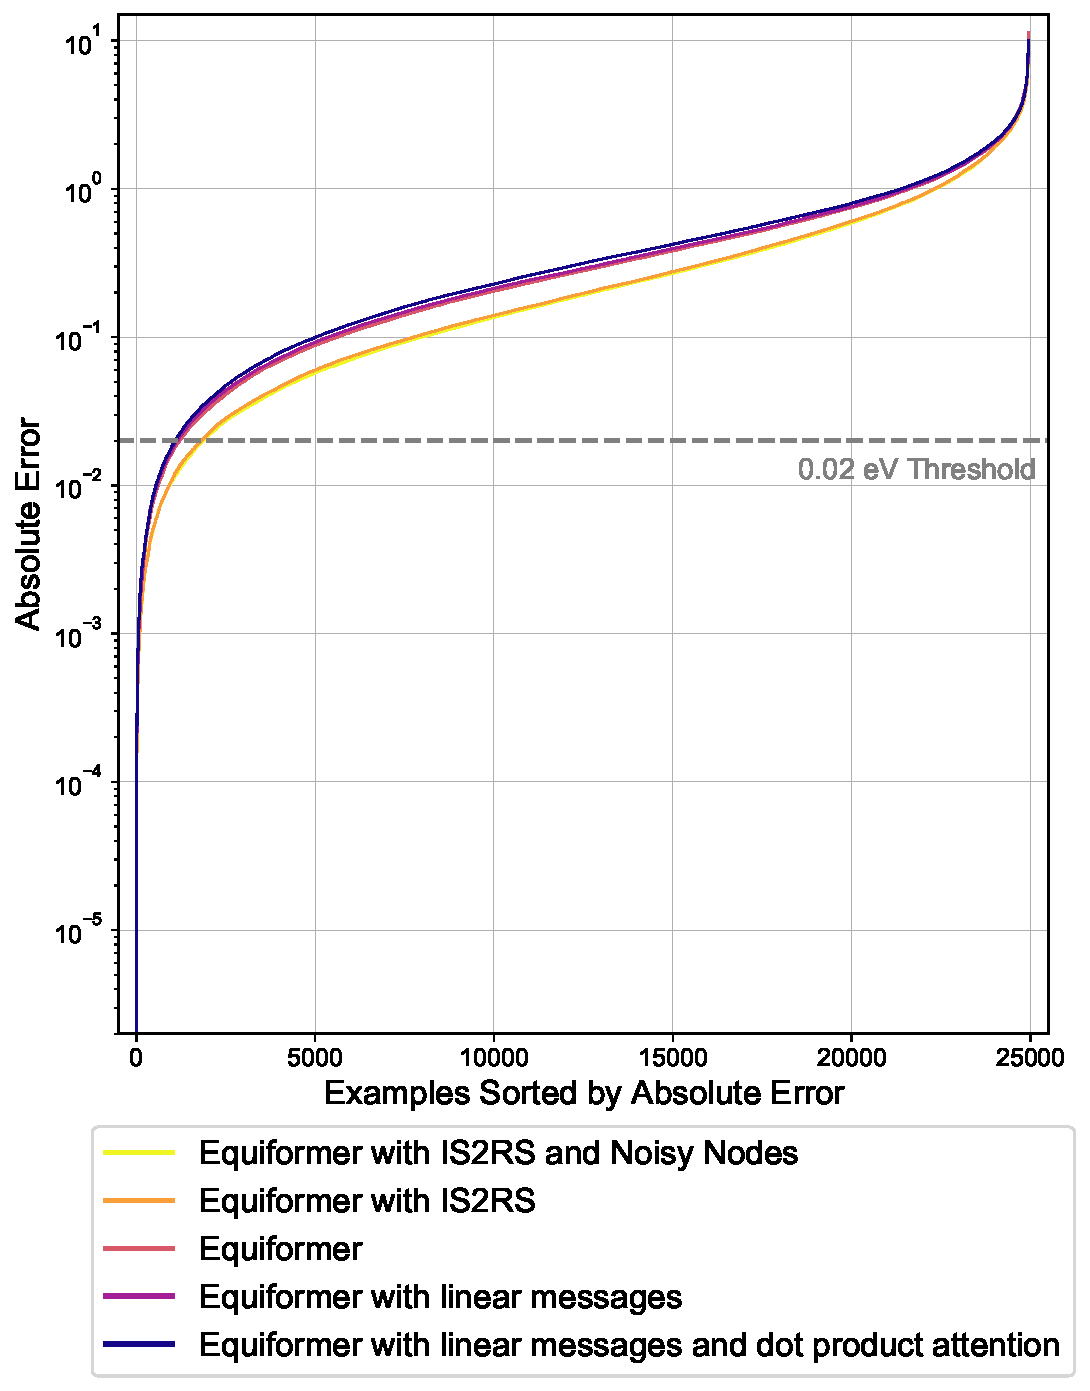
\includegraphics[width=\linewidth]{figure/val_id.pdf}
  \caption{\textbf{ID sub-split.}}
  \vspace{6mm}
  \label{appendix:fig:oc20_val_id}
\end{subfigure}
\begin{subfigure}{.495\textwidth}
  \centering
  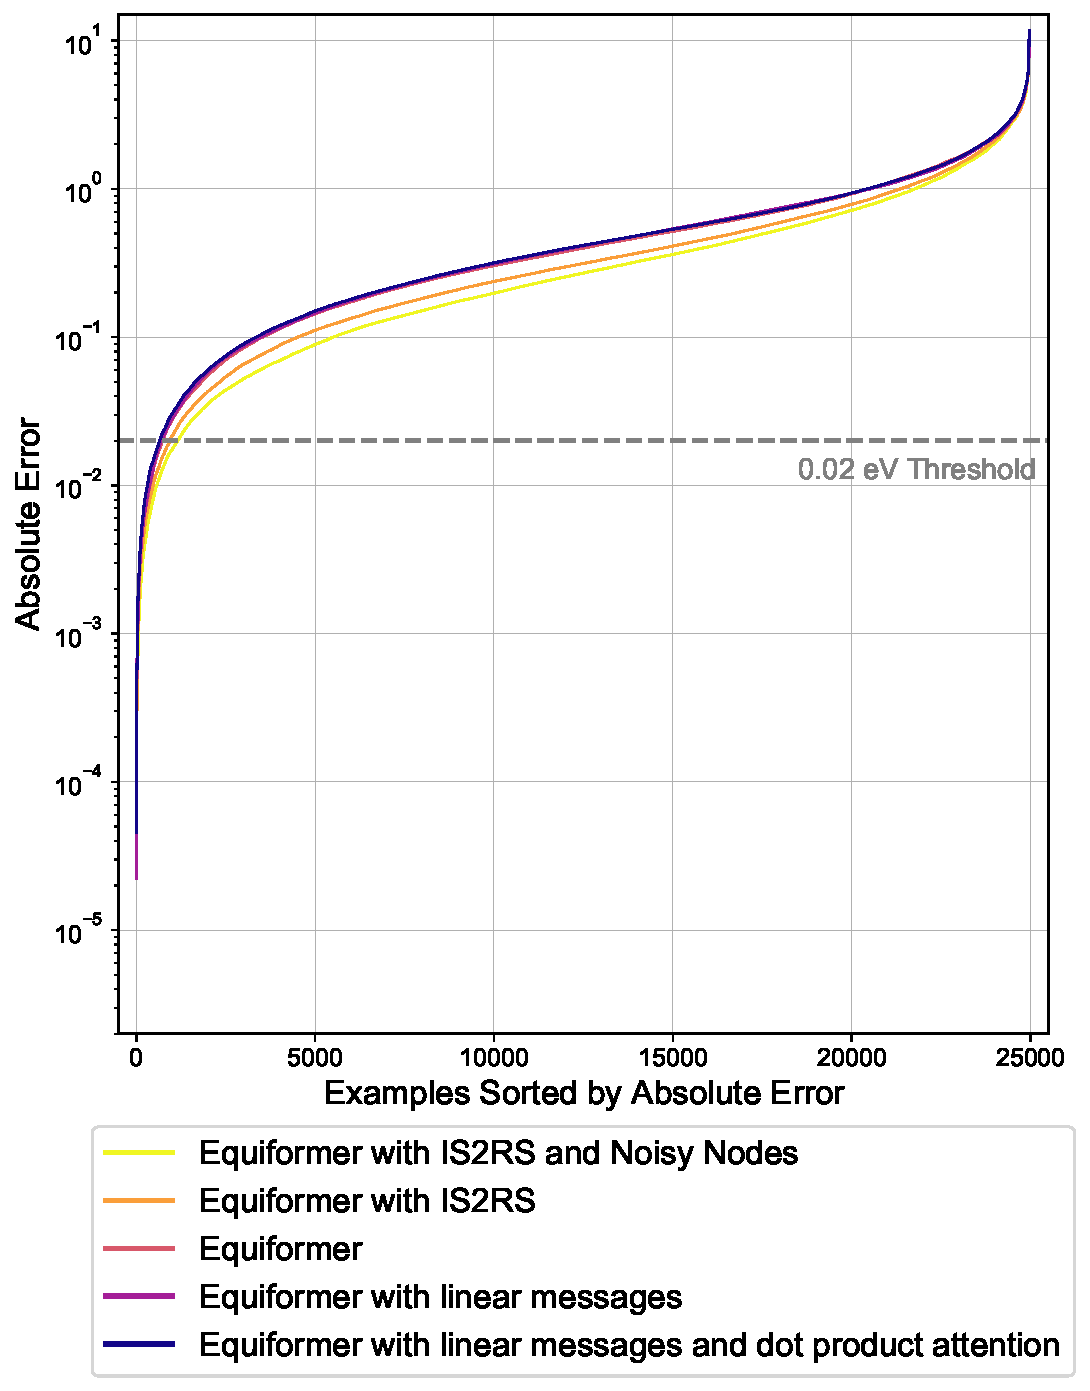
\includegraphics[width=\linewidth]{figure/val_ood_ads.pdf}
  \caption{\textbf{OOD Ads sub-split.}}
  \vspace{6mm}
  \label{appendix:fig:oc20_val_ood_ads}
\end{subfigure}
\begin{subfigure}{.495\textwidth}
  \centering
  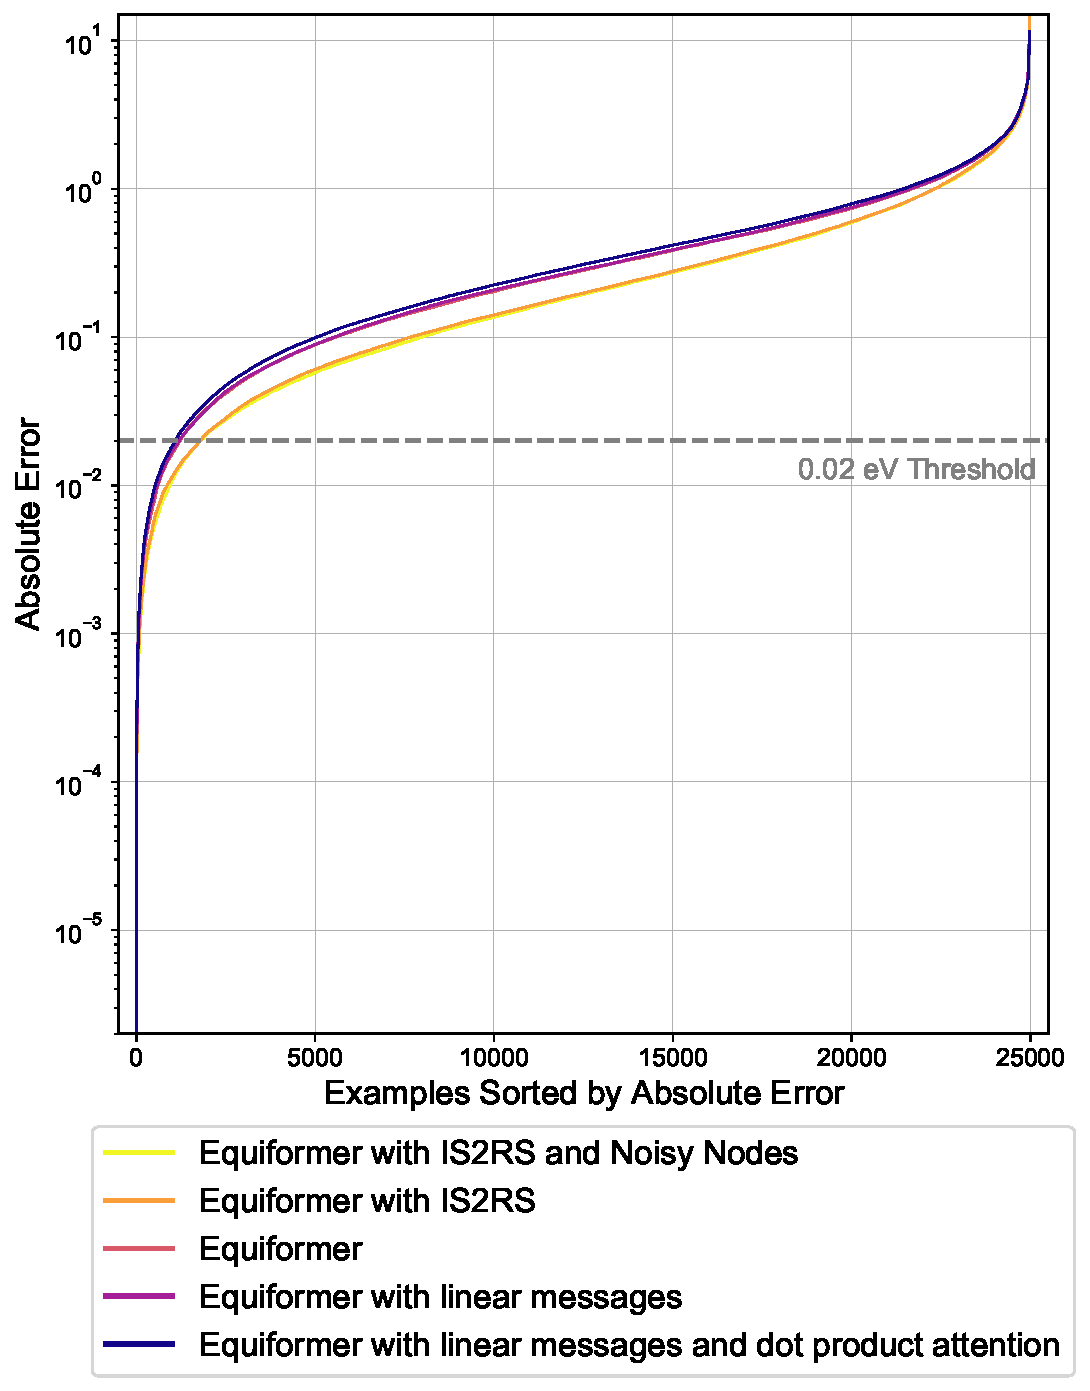
\includegraphics[width=\linewidth]{figure/val_ood_cat.pdf}
  \caption{\textbf{OOD Cat sub-split.}}
  \label{appendix:fig:oc20_val_ood_ads}
\end{subfigure}
\begin{subfigure}{.495\textwidth}
  \centering
  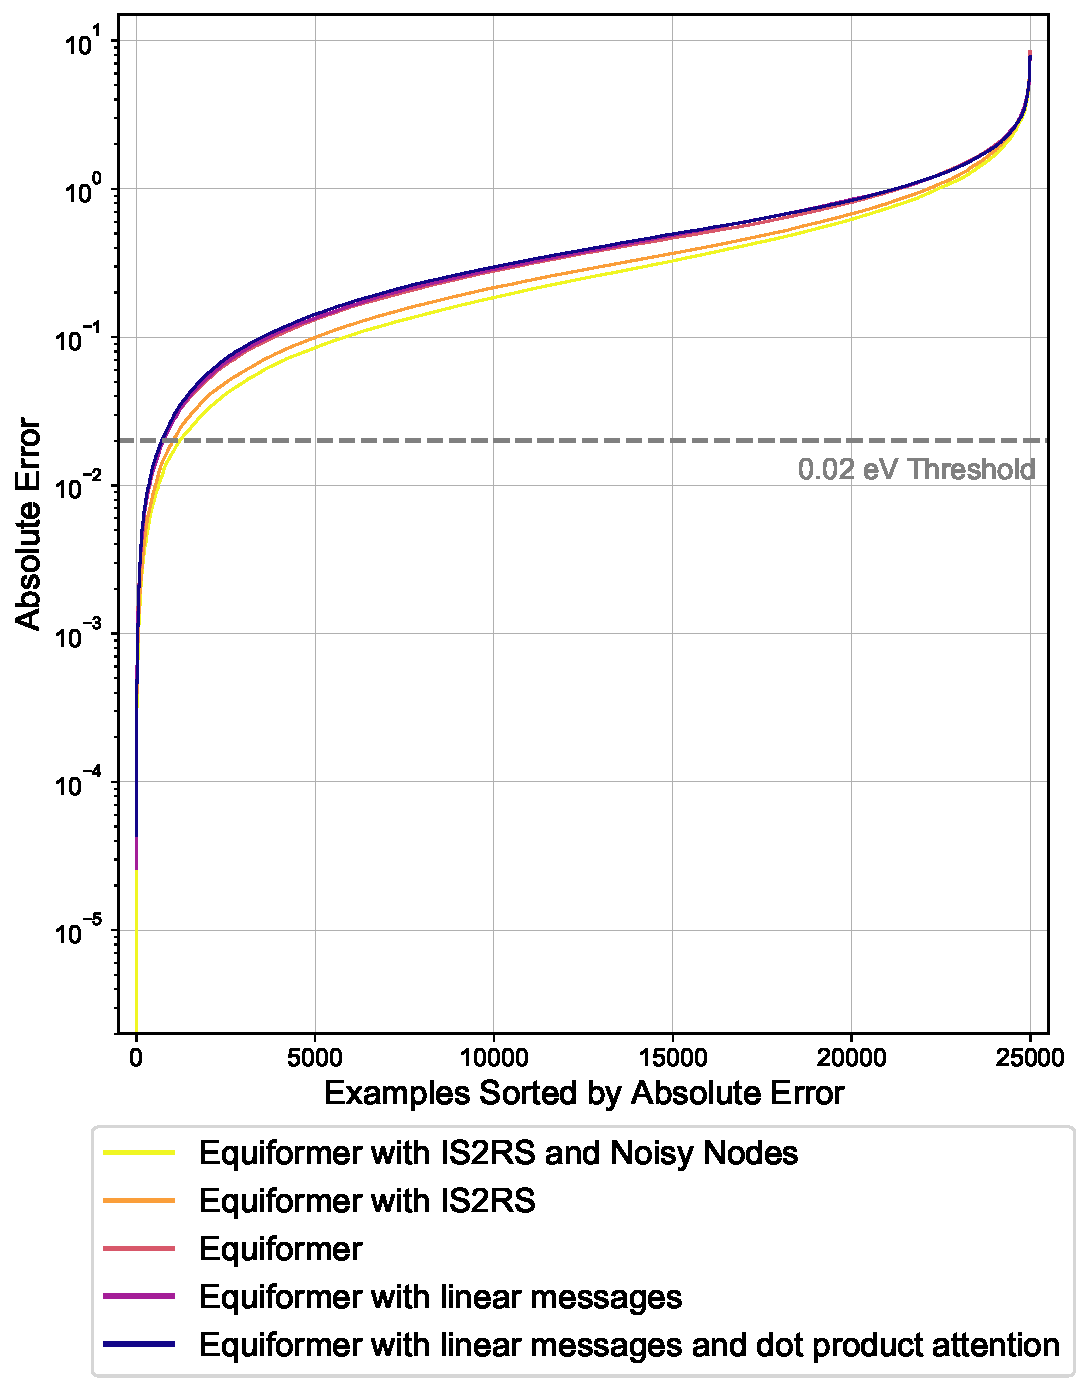
\includegraphics[width=\linewidth]{figure/val_ood_both.pdf}
  \caption{\textbf{OOD Both sub-split.}}
  \label{appendix:fig:oc20_val_ood_ads}
\end{subfigure}
\vspace{4mm}
\caption{\textbf{Error distributions of different Equiformer models on different sub-splits of OC20 IS2RE validation set.} 
%\todo{Examples sorted by error.}
%\todo{Colors of the curves.}
}
\label{appendix:fig:oc20_error_distribution}
\end{figure}

% plot_color_gradients('Perceptually Uniform Sequential',
%                     ['viridis', 'plasma', 'inferno', 'magma', 'cividis'])



